\documentclass[conference]{IEEEtran}

\IEEEoverridecommandlockouts
% The preceding line is only needed to identify funding in the first footnote. If that is unneeded, please comment it out.

% Packages
\usepackage{cite}
\usepackage{enumitem}
\usepackage{amsmath,amssymb,amsfonts}
\usepackage{algorithm}
\usepackage{algorithmic}
\usepackage{graphicx}
\usepackage{textcomp}
\usepackage{xcolor}
\usepackage{forest}
\usetikzlibrary{trees,positioning,shapes,shadows,arrows.meta, calc}
\usepackage{tikz}
\usepackage{adjustbox} % For scaling the figure
\usepackage{url}

% Additional packages for figures and tables
\usepackage{pgfplots}
\usepackage{booktabs}  % For professional tables
\usepackage{colortbl}  % For colored table cells
\usepackage{quantikz}  % For quantum circuits
% \pgfplotsset{compat=1.18}
\usetikzlibrary{shapes.geometric,arrows,positioning,fit,backgrounds,calc,decorations.pathreplacing,decorations.markings,patterns,circuits.logic.US,matrix,chains}

% Custom command for line breaks in author block
\makeatletter
\newcommand{\linebreakand}{%
  \end{@IEEEauthorhalign}
  \hfill\mbox{}\par
  \mbox{}\hfill\begin{@IEEEauthorhalign}
}
\makeatother

% Define quantum computing related colors
\definecolor{qubitblue}{RGB}{70,130,180}
\definecolor{controlred}{RGB}{220,20,60}
\definecolor{aigreen}{RGB}{50,150,50}
\definecolor{quantumpurple}{RGB}{128,0,128}
\definecolor{errororange}{RGB}{255,140,0}

\begin{document}

\title{Quantum Computing Enhanced by Artificial Intelligence: Principles and Applications}

\author{
    \IEEEauthorblockN{
        Benji Peng\textsuperscript{*, a, b},
        Chia Xin Liang \textsuperscript{c},
        Keyu Chen\textsuperscript{a},
        Ziqian Bi\textsuperscript{d}, 
        Ming Liu\textsuperscript{e},
        Yichao Zhang\textsuperscript{f}, \\
        Tianyang Wang\textsuperscript{g},
        Xinyuan Song \textsuperscript{h}
    }
    \IEEEauthorblockA{
        \textsuperscript{a}Georgia Institute of Technology, USA
    }
    \IEEEauthorblockA{
        \textsuperscript{b}AppCubic, USA
    }
    \IEEEauthorblockA{
        \textsuperscript{c}JTB Technology Corp., ROC
    }
    \IEEEauthorblockA{
        \textsuperscript{d}Indiana University, USA
    }
    \IEEEauthorblockA{
        \textsuperscript{e}Purdue University, USA
    }
    \IEEEauthorblockA{
        \textsuperscript{f}The University of Texas at Dallas, USA
    }
    \IEEEauthorblockA{
        \textsuperscript{g}University of Liverpool, UK
    }
    \IEEEauthorblockA{
        \textsuperscript{h}Emory University, USA
    }
    \IEEEauthorblockA{
        *Corresponding Email: benji@appcubic.com
    }
}

\maketitle

\begin{IEEEkeywords}
quantum computing, artificial intelligence, machine learning, neural networks, reinforcement learning, quantum error correction, quantum control
\end{IEEEkeywords}


\begin{abstract}
Artificial intelligence (AI) approaches are transforming quantum computing research across hardware, algorithms, and applications. The high-dimensional nature and unique properties of quantum systems align well with AI's pattern recognition capabilities. This article examines how modern AI techniques advance quantum computing development throughout the computing stack - from hardware design to execution and result interpretation. We explore the mathematical foundations, practical implementations, and emerging opportunities where AI can help overcome key technical barriers in quantum computing advancement.
\end{abstract}


\section{Introduction}
Quantum computing promises computational advantages for specific problems by harnessing quantum mechanical phenomena such as superposition and entanglement \cite{alexeev2021quantum}. As quantum hardware advances from noisy intermediate-scale quantum (NISQ) devices toward fault-tolerant systems, numerous technical challenges emerge across the quantum computing stack - from device physics to algorithm implementation.

Artificial intelligence offers powerful tools for addressing these challenges. The complex, high-dimensional, and non-linear nature of quantum systems makes them particularly amenable to AI approaches \cite{dunjko2023artificial}. Machine learning techniques excel at recognizing patterns in multidimensional spaces and optimizing complex functions - capabilities directly applicable to quantum computing problems.

This article explores applications of AI techniques for enhancing quantum computing development and operation. We focus on how AI accelerates quantum computing research and implementation rather than on quantum computing's potential future impact on AI itself. The content addresses the complete quantum computing workflow, from fundamental AI methods relevant to quantum applications through hardware optimization, circuit synthesis, control systems, error management, and error correction strategies. For each area, we present the mathematical foundations where appropriate and examine how AI techniques provide novel solutions to quantum computing challenges.

\subsection{AI Paradigms for Quantum Computing}

Several key AI paradigms have demonstrated particular relevance to quantum computing challenges. Supervised learning models, trained on labeled data, can predict properties of quantum systems with remarkable accuracy. These methods have proven effective for tasks such as predicting the ground state energies of molecular systems or estimating the fidelity of quantum operations under noise.

Unsupervised learning techniques discover structure in quantum data without explicit labels. Such approaches have been successfully applied to identify patterns in experimental measurement results and to cluster quantum states according to their entanglement properties \cite{janiesch2021machine}.

Reinforcement learning (RL) has emerged as a particularly powerful paradigm for quantum computing \cite{arulkumaran2017deep, shakya2023reinforcement}. By formulating quantum control and optimization as sequential decision processes, RL agents learn optimal policies through direct interaction with quantum systems or their simulations. This approach has proven especially valuable for discovering non-intuitive control strategies that outperform conventional methods.

Deep learning architectures, with their ability to extract hierarchical features from complex data \cite{lecun2015deep}, provide the foundation for many quantum applications. These neural networks can process the high-dimensional data associated with quantum states and processes, enabling more efficient representation and manipulation of quantum information.

Generative models represent another crucial AI approach for quantum computing. These architectures create novel quantum circuits, control sequences, and error correction codes by learning probability distributions over complex quantum objects \cite{bernardo2007generative}. Recent advances in generative models have demonstrated their ability to discover quantum protocols that match or exceed those designed by human experts.

\subsection{Structure of this Article}

The remainder of this article is organized according to the quantum computing workflow. Section 2 examines fundamental AI techniques and their mathematical formulations relevant to quantum computing applications. Section 3 explores quantum hardware optimization, including system identification, device design, and pulse optimization. Section 4 addresses circuit synthesis and optimization, focusing on AI methods for transforming abstract algorithms into efficient implementations. Section 5 covers quantum control and error management during execution, while Section 6 explores AI approaches for error correction and mitigation. Finally, Sections 7 and 8 discuss emerging research directions and summarize the key insights regarding the synergy between AI and quantum computing. 

\section{AI Fundamentals for Quantum Computing}
AI techniques are particularly well-suited for quantum computing challenges due to their ability to handle high-dimensional data and complex optimization problems. This section examines the mathematical principles of key AI approaches and their quantum computing applications.

\subsection{Neural Networks for Quantum Systems}

Neural networks form the foundation of many AI approaches in quantum computing. A feed-forward neural network with $L$ layers can be expressed as a composition of functions:

\begin{equation}
f(x) = (f_L \circ f_{L-1} \circ \cdots \circ f_1)(x)
\end{equation}

where each layer $f_i(x) = \sigma(W_i x + b_i)$ applies a linear transformation followed by a non-linear activation function $\sigma$. The universal approximation theorem \cite{hornik1989multilayer} guarantees that such networks can represent arbitrarily complex functions - a critical property for modeling quantum phenomena.

\subsubsection{Architecture Specialization for Quantum Tasks}

Several neural network architectures have been specialized for quantum computing applications. Convolutional Neural Networks (CNNs) exploit spatial locality in quantum data, making them particularly effective for processing quantum state tomography results and error syndromes in topological codes. Their translation invariance properties align well with the spatial structure of many quantum error correction codes.

Recurrent Neural Networks (RNNs) excel at modeling temporal dynamics in quantum systems \cite{banchi2018modelling}. These architectures maintain an internal state that captures information about past inputs, enabling them to process sequence data such as quantum control pulses or time-dependent measurement records. Long Short-Term Memory (LSTM) networks and Gated Recurrent Units (GRUs) have proven especially effective for quantum control optimization tasks where temporal correlations span multiple timescales.

Graph Neural Networks (GNNs) process data structured as graphs, making them ideal for quantum circuits represented as directed acyclic graphs. In these applications, nodes represent quantum gates or operations, while edges represent qubit connections or information flow. GNNs have demonstrated significant advantages for circuit optimization and quantum architecture design by directly operating on the circuit's graph structure.

Transformer architectures, which leverage attention mechanisms to capture long-range dependencies, have recently been applied to quantum circuit design and control sequence optimization. These models can identify correlations between operations separated by significant circuit depth, enabling more efficient circuit synthesis and optimization.

\subsection{Reinforcement Learning for Quantum Control}

Reinforcement learning formulates quantum control as a Markov decision process (MDP), where states $s \in \mathcal{S}$ represent quantum system configurations, actions $a \in \mathcal{A}$ correspond to control operations, transition dynamics $P(s'|s,a)$ follow quantum mechanical laws, and reward function $R(s,a,s')$ measures control quality (e.g., gate fidelity).

RL aims to find a policy $\pi: \mathcal{S} \rightarrow \mathcal{A}$ maximizing expected cumulative reward:

\begin{equation}
J(\pi) = \mathbb{E}_{\tau \sim \pi}\left[\sum_{t=0}^{T} \gamma^t R(s_t, a_t, s_{t+1})\right]
\end{equation}

where $\tau$ represents a trajectory of states and actions, and $\gamma$ is a discount factor.

\subsubsection{RL Advantages for Quantum Applications}

For quantum control \cite{bukov2018reinforcement}, RL offers several significant advantages over traditional optimization approaches. First, RL enables exploration of non-intuitive control strategies beyond traditional approaches derived from analytical methods. This has led to the discovery of control protocols that achieve higher fidelities and shorter gate times than previously thought possible.

Second, RL methods demonstrate remarkable adaptability to quantum system variations and uncertainties. By incorporating system fluctuations into the training process, RL agents learn robust policies that maintain performance despite fabrication imperfections or environmental drift. This robustness is particularly valuable for real-world quantum hardware where ideal parameters are rarely achieved.

Third, RL provides end-to-end optimization without requiring analytical gradients of the objective function with respect to control parameters. This gradient-free approach is especially valuable for quantum systems where the exact relationship between controls and performance may be complex or unknown. Finally, RL algorithms can directly incorporate physical constraints into the learning process, ensuring that generated control sequences respect hardware limitations such as bandwidth constraints or maximum field strengths.

\subsection{Generative Models for Quantum States and Circuits}

Generative models learn probability distributions over quantum objects such as states, circuits, or control sequences. These models enable the creation of novel quantum protocols that may exceed human-designed approaches in efficiency or performance.

\subsubsection{Variational Autoencoders}

Variational Autoencoders (VAEs) provide a framework for learning compressed representations of quantum data. These models encode quantum states or circuits into a lower-dimensional latent space via an encoder network $q_\phi(z|x)$ and decode via $p_\theta(x|z)$, trained to maximize:

\begin{equation}
\mathcal{L}(\theta, \phi; x) = \mathbb{E}_{q_\phi(z|x)}[\log p_\theta(x|z)] - D_{KL}(q_\phi(z|x) || p(z))
\end{equation}

The first term encourages accurate reconstruction of input data, while the second term, the Kullback-Leibler divergence, ensures the latent space follows a prior distribution $p(z)$, typically a standard normal distribution. In quantum computing applications, VAEs have been used to discover efficient circuit representations and for quantum state compression.

\subsubsection{Adversarial and Diffusion Models}

Generative Adversarial Networks (GANs) employ a competitive training process between a generator $G(z)$ and discriminator $D(x)$. The generator creates quantum circuits or states from random noise, while the discriminator attempts to distinguish these generated samples from real examples. Through this adversarial process, the generator learns to produce increasingly realistic quantum objects. GANs have been applied to generate quantum circuits for specific tasks and to create synthetic quantum data for training other machine learning models.

Diffusion models represent a more recent approach to quantum circuit generation \cite{furrutter2024quantum}. These models work by learning to reverse a gradual noising process, starting from a complex circuit and progressively simplifying it through noise addition. By inverting this process, diffusion models can generate high-quality quantum circuits starting from random noise. Recent work has demonstrated that diffusion models can discover circuit implementations that match or exceed those designed by human experts, particularly for complex unitary operations.

\subsection{Transfer Learning for Quantum Tasks}

Transfer learning addresses the challenge of limited training data in quantum computing by adapting models trained on one quantum task to another related task. For a source task $\mathcal{T}_S$ and target task $\mathcal{T}_T$, knowledge transfer occurs when:

\begin{equation}
P(Y_T | X_T) = \int P(Y_T | X_T, K) P(K | \mathcal{T}_S) dK
\end{equation}

where $K$ represents transferable knowledge.

This approach has proven valuable for transferring learned representations between similar quantum hardware platforms. For example, models trained on simulated quantum devices can be fine-tuned with limited data from real hardware, significantly accelerating the development of hardware-specific control strategies. Similarly, control policies learned on smaller quantum systems can be transferred to larger systems, helping address the exponential scaling challenge of quantum simulation.

Transfer learning has also demonstrated success in adapting error correction decoders to larger code distances. By training on smaller, tractable codes and transferring knowledge to larger codes, researchers have developed decoders that scale more efficiently than those trained from scratch on each code size. This scalability is crucial for practical quantum error correction, where code distances must increase as quantum computers grow in size.

These mathematical frameworks provide powerful tools for addressing quantum computing challenges, with implementations demonstrating clear advantages over traditional methods across multiple domains of the quantum computing stack. 

\section{Quantum Hardware Optimization}
Quantum hardware development presents unique optimization challenges that AI techniques can effectively address. This section examines key applications of AI for quantum hardware characterization and design.

\subsection{Hamiltonian Learning and System Identification}

Identifying quantum system Hamiltonians from experimental data is a fundamental challenge in quantum hardware development. For a quantum system with Hamiltonian $H = \sum_i \alpha_i H_i$, where $\{H_i\}$ are known operators and $\{\alpha_i\}$ are unknown parameters, machine learning approaches can efficiently estimate these parameters from limited measurement data.

Bayesian methods have proven particularly effective for Hamiltonian learning \cite{wiebe2014hamiltonian}, with posterior parameter updates given by:

\begin{equation}
P(\alpha | D) \propto P(D | \alpha) P(\alpha)
\end{equation}

where $D$ represents measurement outcomes. The likelihood function $P(D | \alpha)$ encodes the probability of observing specific measurement results given particular Hamiltonian parameters, while the prior $P(\alpha)$ incorporates existing knowledge about these parameters. 

Neural networks can accelerate this process by learning mappings from measurement data to Hamiltonian parameters, enabling rapid system identification. These approaches are especially valuable when the relationship between observed data and underlying parameters is complex or when experimental time is limited. For example, convolutional neural networks have been applied to extract two-qubit coupling strengths from time-series measurement data with significantly fewer experimental runs than traditional tomography methods.

\subsection{Quantum Device Design Optimization}

AI techniques enable automated exploration of the vast design space for quantum devices. This automation has accelerated progress across multiple quantum computing platforms by efficiently identifying promising design configurations.

\subsubsection{Material Parameter Optimization}

Material selection and parameter tuning represent critical challenges in quantum device design. Machine learning models can predict how material choices affect qubit properties by learning from fabrication data and physical simulations. For superconducting qubits, neural networks have been trained to predict coherence times based on material composition, fabrication parameters, and geometric design. These models enable rapid evaluation of design alternatives without requiring time-consuming fabrication and testing of each variant.

Similarly, for spin qubits in semiconductors, Gaussian process regression models have been employed to optimize doping profiles and gate geometries. By systematically exploring the relationship between design parameters and qubit performance metrics such as gate fidelity and coherence time, these models accelerate the search for optimal configurations.

\subsubsection{Layout and Topology Optimization}

The spatial arrangement of qubits and control lines significantly impacts device performance, particularly for superconducting and ion trap quantum computers. Traditional optimization approaches struggle with this high-dimensional problem due to the exponential growth of the design space with qubit count.

Genetic algorithms and reinforcement learning offer powerful alternatives for layout optimization. These approaches can discover configurations that minimize crosstalk while maximizing connectivity and operational fidelity. Recent work has demonstrated reinforcement learning agents that design trap layouts for ion-based quantum computers, optimizing for both quantum gate fidelity and classical control complexity.

For superconducting quantum processors, graph neural networks have proven effective for predicting crosstalk patterns based on device topology. These models inform the design of chip layouts that minimize unwanted qubit interactions while respecting fabrication constraints. The resulting designs often exhibit counter-intuitive geometric arrangements that would be difficult to discover through manual design processes.

\subsubsection{Fabrication Process Optimization}

Quantum device manufacturing involves complex fabrication processes with numerous parameters that influence device performance. Neural networks can learn relationships between fabrication parameters and resulting device properties, enabling targeted improvements in manufacturing processes.

Convolutional neural networks have been applied to analyze scanning electron microscope images of fabricated devices, identifying defects and predicting their impact on qubit performance. This automated analysis accelerates the fabrication feedback loop, allowing rapid iteration on process parameters. Similarly, Bayesian optimization approaches have been employed to tune lithography and etching parameters for maximizing device yield and consistency.

\subsection{Pulse Optimization for Gate Implementation}

Implementing high-fidelity quantum gates requires precisely designed control pulses. For a target unitary operation $U$, the control problem seeks a time-dependent Hamiltonian $H(t) = H_0 + \sum_j c_j(t) H_j$ producing an evolution operator $U_T$ that maximizes fidelity:

\begin{equation}
\mathcal{F}(U, U_T) = \left|\frac{1}{d}\text{Tr}(U^\dagger U_T)\right|^2
\end{equation}

where $d$ is the Hilbert space dimension. Conventional approaches to pulse optimization include techniques such as GRAPE (Gradient Ascent Pulse Engineering) and CRAB (Chopped Random Basis), which use gradient-based optimization to find effective pulse shapes.

Reinforcement learning algorithms have demonstrated remarkable success in this domain \cite{ding2021breaking}, discovering pulse shapes that achieve higher fidelities than conventional methods. These machine learning approaches have identified control protocols that reduce gate duration beyond theoretical limits of adiabatic control, potentially enabling more operations within coherence time constraints. The RL-designed pulses also demonstrate enhanced robustness against experimental variations, maintaining high performance despite fluctuations in system parameters.

Another significant advantage of AI-designed pulses is their ability to minimize leakage to non-computational states. By incorporating leakage penalties directly into the optimization objective, reinforcement learning agents learn control strategies that confine dynamics to the computational subspace, addressing a common challenge in many qubit implementations.

For parametrized pulse shapes, gradient-based optimization using differentiable quantum simulators can efficiently find optimal parameters. However, RL approaches often discover entirely new pulse shapes that gradient descent might miss due to local optima. This global exploration capability represents a key advantage of machine learning for quantum control optimization.

\begin{figure}[!t]
\centering
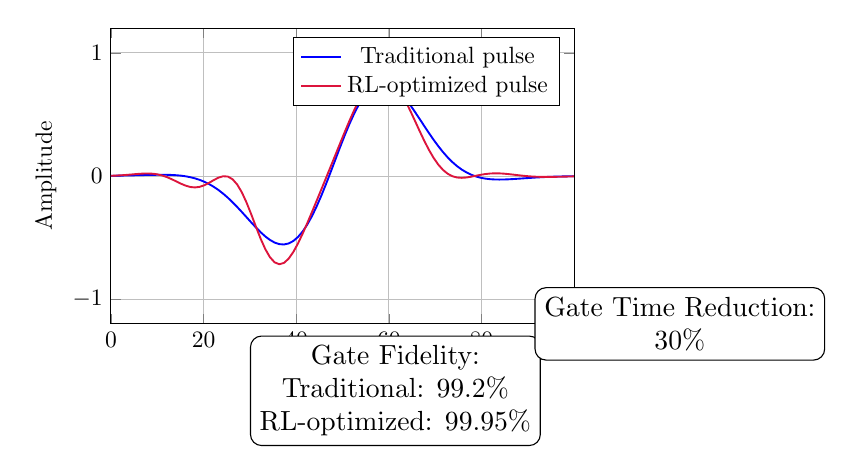
\begin{tikzpicture}[scale=0.85]
    % Set up the coordinate system
    \begin{axis}[
        xlabel={Time (ns)},
        ylabel={Amplitude},
        xmin=0, xmax=100,
        ymin=-1.2, ymax=1.2,
        legend pos=north east,
        grid=both,
        width=8.5cm,
        height=6cm,
    ]
    
    % Traditional DRAG pulse
    \addplot[thick, blue, domain=0:100, samples=100] {exp(-(x-50)^2/400)*cos(deg(0.1*x))};
    
    % AI-optimized pulse (more complex shape with higher fidelity)
    \addplot[thick, controlred, domain=0:100, samples=100] {exp(-(x-50)^2/400)*cos(deg(0.1*x)) + 0.2*sin(deg(0.3*x))*exp(-(x-30)^2/200) - 0.15*sin(deg(0.2*x))*exp(-(x-70)^2/200)};
    
    % Add legend
    \legend{Traditional pulse, RL-optimized pulse};
    
    \end{axis}
    
    % Add fidelity information
    \node[align=center, fill=white, draw=black, rounded corners] at (4.25,-1) {Gate Fidelity:\\Traditional: 99.2\%\\RL-optimized: 99.95\%};
    
    % Add gate time reduction
    \node[align=center, fill=white, draw=black, rounded corners] at (8.5,0) {Gate Time Reduction:\\30\%};
    
\end{tikzpicture}
\caption{Comparison of traditional and reinforcement learning (RL) optimized control pulses for a single-qubit gate. The RL-optimized pulse (red) achieves higher fidelity while requiring shorter implementation time compared to the traditional pulse shape (blue). The complex shape discovered by RL includes features that counteract specific noise sources and leakage to non-computational states.}
\label{fig:pulse_optimization}
\end{figure}

\subsection{Noise Characterization and Mitigation}

AI methods effectively characterize and mitigate noise in quantum hardware. The process matrix $\chi$ describing a noisy quantum channel can be efficiently learned from experimental data using maximum likelihood estimation enhanced by neural networks. These learned noise models provide crucial information for designing error mitigation strategies and optimizing quantum algorithms for specific hardware.

Bayesian inference approaches can model complex noise correlations with far fewer measurements than traditional tomography requires. By incorporating prior knowledge about the physical system and updating this understanding based on measurement results, Bayesian methods construct detailed noise models with practical measurement budgets. Gaussian process regression has proven particularly effective for modeling spatiotemporal noise correlations across multi-qubit devices.

Neural network classifiers have been applied to distinguish different noise mechanisms based on their signatures in measurement data. This classification enables targeted mitigation strategies for specific noise types rather than generic approaches. For example, different techniques can be employed depending on whether coherent control errors or decoherence effects dominate in a particular device.

The resulting noise models enable the design of optimized error mitigation strategies specific to each quantum device's characteristics. These tailored approaches significantly outperform generic error mitigation techniques, improving computational results without requiring full quantum error correction. 

\section{Circuit Synthesis and Optimization}
Before executing quantum algorithms, several preprocessing steps can significantly impact performance. This section explores how AI is enhancing these preparatory phases.

\subsection{Quantum Circuit Synthesis}
Converting algorithms to efficient quantum circuits presents numerous challenges that AI methods are helping to address.

\subsubsection{Unitary Synthesis}
AI techniques are providing new approaches to decomposing arbitrary unitary operations into sequences of available gates, often finding more efficient implementations than traditional decomposition methods.

\subsubsection{AI Models to Generate Compact Circuits}
Recent work with generative models has shown promise in creating more compact circuit representations, potentially reducing resource requirements for quantum algorithms.

\subsection{Circuit Parameter Learning and Parameter Transfer}
For parameterized quantum circuits, finding optimal parameters is challenging due to issues like barren plateaus. AI methods can help navigate these complex optimization landscapes more effectively.

\subsection{State Preparation}
Preparing specific quantum states efficiently is crucial for many algorithms. AI approaches are helping develop improved state preparation protocols that require fewer operations and are more robust to noise. 

\section{Quantum Control and Error Management}
Quantum systems require precise control to maintain coherence and execute operations with high fidelity. AI techniques offer significant advantages for both offline control optimization and real-time error management.

\subsection{Optimal Control Theory}

Quantum optimal control seeks time-dependent control fields $\{c_j(t)\}$ that drive a quantum system governed by the Hamiltonian:

\begin{equation}
H(t) = H_0 + \sum_j c_j(t) H_j
\end{equation}

where $H_0$ is the drift Hamiltonian and $\{H_j\}$ are control Hamiltonians. The goal is to evolve the system from an initial state $\rho_0$ to a target state $\rho_T$ or to implement a target unitary $U_T$.

Traditional approaches like GRAPE (Gradient Ascent Pulse Engineering) use gradient information to optimize control parameters. AI methods extend these capabilities through model-free optimization techniques. Reinforcement learning agents can discover high-fidelity control sequences without explicit system models \cite{bukov2018reinforcement}, enabling control optimization even when accurate system models are unavailable or prohibitively complex.

Neural network controllers exhibit remarkable robustness to uncertainty in system parameters. By incorporating parameter variations during training, these controllers learn policies that maintain performance despite fabrication imperfections or environmental fluctuations. This robustness is particularly valuable for scaling quantum systems, where consistent performance across multiple qubits with varying parameters presents a significant challenge.

One of the most compelling demonstrations of AI-based quantum control is the discovery of protocols that exceed the speed limits of adiabatic control \cite{ding2021breaking}. While conventional adiabatic approaches require slow evolution to avoid excitations to unwanted states, RL agents have identified non-adiabatic protocols that achieve the same final states in significantly less time. These counter-intuitive control strategies can enable more operations within coherence time constraints, addressing a fundamental limitation of quantum computing systems.

\subsection{Real-time Adaptive Control}

Real-time control adjusts operations based on continuous measurement feedback. For a partially observable quantum system, the control problem becomes a partially observable Markov decision process (POMDP) where states represent quantum density matrices $\rho$, actions are control operations, and observations are measurement outcomes with probability distributions determined by quantum mechanics.

Deep reinforcement learning strategies for this POMDP can be formulated using recurrent neural networks that maintain internal representations of quantum state estimates. The resulting controllers can generate control policies conditioned on measurement history:

\begin{equation}
\pi(a_t | o_1, o_2, \ldots, o_t) = \text{RNN}(o_t, h_{t-1})
\end{equation}

where $o_t$ are observations, $a_t$ are actions, and $h_t$ is the hidden state of the RNN.

Adaptive control has demonstrated particular value for non-Markovian quantum systems, where environmental memory effects create temporal correlations in system dynamics. Recurrent neural networks can capture these temporal correlations and adjust control strategies accordingly, outperforming memoryless controllers. For example, RNN controllers have been applied to superconducting qubits subject to $1/f$ noise, adaptively compensating for low-frequency drift that would otherwise cause gate errors to accumulate.

Another promising application is measurement-based feedback for quantum error correction. Neural network policies can determine optimal correction operations based on syndrome measurement sequences, accounting for both the observed error syndromes and the statistical correlations between errors. These adaptive approaches demonstrate higher error correction thresholds than standard table-based decoders, particularly for complex noise models with temporal and spatial correlations.

\begin{figure}[!t]
\centering
\begin{tikzpicture}[node distance=1.8cm, auto, >=latex', scale=0.8, transform shape]
    % Quantum System
    \node [draw, rectangle, rounded corners, minimum width=3cm, minimum height=1.5cm, fill=quantumpurple!10] (system) {Quantum System};
    
    % Measurement Device
    \node [draw, rectangle, below of=system, minimum width=2.5cm, minimum height=1cm] (measure) {Measurement};
    
    % RNN Controller
    \node [draw, rectangle, rounded corners, left of=system, node distance=5cm, minimum width=2.5cm, minimum height=3.5cm, fill=controlred!10] (controller) {RNN Controller};
    
    % Hidden state
    \node [draw, rectangle, below of=controller, node distance=2.5cm, minimum width=2cm, minimum height=0.8cm, fill=controlred!30] (hidden) {Hidden State $h_t$};
    
    % Control Pulse
    \node [draw, rectangle, above of=system, minimum width=2cm, minimum height=0.8cm] (pulse) {Control Pulse};
    
    % Arrows
    \draw[->] (controller) -- node[above] {$a_t$} (system);
    \draw[->] (system) -- node[right] {} (measure);
    \draw[->] (measure) -- node[below] {$o_t$} ++(-3,0) |- (controller);
    \draw[->] (controller) -- node[left] {} (hidden);
    \draw[->] (hidden) -- ++(-1,0) |- node[left, near start] {$h_{t-1}$} (controller);
    \draw[->] (controller) -- ++(-1,0) |- node[left] {$c_j(t)$} (pulse);
    \draw[->] (pulse) -- (system);
    
    % System state
    \node[draw, align=center, fill=quantumpurple!5] at (5,0) {System State $\rho_t$\\$\ket{\psi_t}$};
    \draw[->] (system) -- (5,0);
    
    % Noise
    \draw[snake=snake, segment amplitude=0.2mm, segment length=1mm, very thick, decorate, ->] (3.5,2) -- (system);
    \node[right] at (3.5,2) {Noise};
    
    % Policy function
    \node[draw, align=center, fill=controlred!5, below of=controller, node distance=4.5cm] 
        (policy) {$\pi(a_t | o_1, o_2, \ldots, o_t) = \text{RNN}(o_t, h_{t-1})$};
    \draw[->, dashed] (hidden) -- (policy);
\end{tikzpicture}
\caption{Recurrent neural network (RNN) based adaptive quantum control. The RNN controller processes measurement observations $o_t$ and maintains an internal hidden state $h_t$ representing its belief about the quantum system state. At each timestep, the controller outputs control actions $a_t$ that generate pulses $c_j(t)$ applied to the quantum system. This closed-loop control enables adaptation to system variations and environmental noise.}
\label{fig:rnn_control}
\end{figure}

\subsection{Multi-qubit Operation Scheduling}

Executing multiple operations across a quantum processor requires sophisticated scheduling to minimize crosstalk and maximize parallelism. Machine learning approaches formulate this as a constrained optimization problem:

\begin{equation}
\min_{\{t_i\}} \sum_i w_i t_i \quad \text{subject to constraints on overlapping operations}
\end{equation}

where $t_i$ represents the start time of operation $i$ and $w_i$ its priority weight.

AI schedulers consider hardware-specific constraints such as control line bandwidth limitations, which restrict simultaneous operations on qubits sharing control infrastructure. They also account for crosstalk between neighboring qubits, which can cause unintended interactions when gates are executed in parallel. By learning from simulation and experimental data, these schedulers develop sophisticated models of inter-qubit interference and optimize operation timing to minimize these effects.

Time-dependent noise characteristics present another scheduling challenge that machine learning approaches effectively address. Many quantum systems exhibit periodic noise fluctuations due to environmental factors or control system limitations. AI schedulers learn these temporal patterns and preferentially schedule high-precision operations during low-noise windows, significantly improving overall computational fidelity.

Variability in operation fidelities across different qubits and gate types also influences optimal scheduling decisions. Reinforcement learning agents learn to prioritize more reliable operations and allocate more precise qubits to critical computational paths, maximizing the probability of successful algorithm execution. This dynamic resource allocation improves computational results without requiring hardware modifications.

\subsection{In-situ Calibration and Drift Compensation}

Quantum systems exhibit parameter drift over time, requiring continuous recalibration. AI techniques enable efficient in-situ calibration through Bayesian experimental design, which selects optimal calibration experiments to maximize information gain. By modeling the uncertainty in system parameters and choosing measurements that most effectively reduce this uncertainty, Bayesian approaches minimize the time spent on calibration procedures.

Online learning approaches continuously update system models based on observed performance during computation. Rather than treating calibration as a separate procedure, these techniques integrate parameter estimation into regular operation, detecting and compensating for drift in real-time. For example, Kalman filter-based approaches have been implemented to track qubit frequency drift in superconducting systems, applying compensating fields without interrupting computation.

Predictive maintenance represents another valuable application of AI for quantum control systems. By analyzing temporal patterns in system parameters, machine learning models can forecast imminent parameter drift and schedule preventive recalibration before performance degrades significantly. These predictive approaches minimize unexpected computational failures and optimize the allocation of calibration time.

These control techniques significantly enhance quantum computer performance by optimizing hardware operation at multiple timescales - from nanosecond pulse shaping to millisecond measurement feedback and hour-to-hour drift compensation. The integration of machine learning throughout the control stack enables more efficient utilization of quantum coherence, ultimately improving computational capabilities. 

\section{Error Correction and Mitigation}
Error management is essential for reliable quantum computation. This section examines AI approaches for both error correction and mitigation.

\subsection{Neural Decoders for Quantum Error Correction}
Quantum error correction (QEC) detects and corrects errors through syndrome measurements. For a stabilizer code with stabilizer group $\mathcal{S}$, the decoding problem involves:

\begin{enumerate}
    \item Measuring syndrome bits $s_i = \langle \psi | S_i | \psi \rangle$ for stabilizers $S_i \in \mathcal{S}$
    \item Inferring the most likely error $E$ given syndrome pattern $s$: $P(E|s)$
    \item Applying the appropriate recovery operation $R$
\end{enumerate}

Neural network decoders frame this as a classification problem, mapping syndromes to recovery operations:

\begin{equation}
f_\theta: \{0,1\}^m \rightarrow \mathcal{P}^n
\end{equation}

where $m$ is the number of syndrome bits, $n$ is the number of physical qubits, and $\mathcal{P}^n$ is the Pauli group on $n$ qubits.

AI approaches offer several advantages:

\begin{itemize}
    \item \textbf{Speed}: Neural decoders can achieve microsecond-scale decoding latency, critical for real-time error correction
    
    \item \textbf{Adaptability}: Models can be trained on device-specific noise profiles rather than assuming idealized noise models
    
    \item \textbf{Scalability}: Architecture designs like convolutional decoders scale efficiently to larger code distances
\end{itemize}

Recent implementations have demonstrated neural decoders with performance approaching or exceeding traditional algorithms like minimum-weight perfect matching, but with significantly reduced computational overhead.

\subsection{Error Correction Code Discovery}
The search for optimal quantum error correction codes presents a complex discrete optimization problem. AI methods explore this space through:

\begin{itemize}
    \item \textbf{Reinforcement learning}: Agents that iteratively construct stabilizer sets, receiving rewards based on code distance and rate
    
    \item \textbf{Genetic algorithms}: Evolutionary approaches that "breed" promising codes to discover improved variants
    
    \item \textbf{Autoencoder architectures}: Neural networks that discover efficient encodings into protected subspaces
\end{itemize}

These approaches have discovered codes with improved distance properties and efficient encoding/decoding circuits tailored to specific hardware constraints.

\subsection{Error Mitigation Techniques}
For near-term quantum devices without full error correction, error mitigation techniques improve computational results. AI enhances these approaches through:

\begin{itemize}
    \item \textbf{Zero-noise extrapolation}: Machine learning models can predict zero-noise limits from measurements at different noise levels:
    
    \begin{equation}
    \langle O \rangle_{\text{ideal}} \approx f_\theta(\langle O \rangle_{\lambda_1}, \langle O \rangle_{\lambda_2}, \ldots, \langle O \rangle_{\lambda_k})
    \end{equation}
    
    where $\langle O \rangle_{\lambda_i}$ represents expectation values at noise scale $\lambda_i$.
    
    \item \textbf{Quantum subspace expansion}: Neural networks can identify optimal subspaces that minimize error effects
    
    \item \textbf{Measurement error mitigation}: ML models learn calibration matrices that correct for readout errors:
    
    \begin{equation}
    \vec{p}_{\text{true}} = A^{-1} \vec{p}_{\text{measured}}
    \end{equation}
    
    where $A$ is the calibration matrix and $\vec{p}$ represents measurement outcome probabilities
\end{itemize}

\subsection{Adaptive Measurement and Tomography}
AI techniques enable more efficient quantum state characterization through:

\begin{itemize}
    \item \textbf{Bayesian experimental design}: Selecting optimal measurements to maximize information gain about quantum states
    
    \item \textbf{Compressed sensing}: Reconstructing quantum states from an incomplete set of measurements, formulated as:
    
    \begin{equation}
    \min_\rho \|\rho\|_1 \quad \text{subject to} \quad \|y - \mathcal{A}(\rho)\|_2 < \epsilon
    \end{equation}
    
    where $y$ represents measurement outcomes, $\mathcal{A}$ is the measurement operator, and $\rho$ is the density matrix
    
    \item \textbf{Neural tomography}: Networks that directly map measurement statistics to density matrix estimates
\end{itemize}

The integration of these error correction and mitigation techniques, enhanced by AI, enables more reliable computation on both current and future quantum hardware. 
% The content of this file has been integrated into the error_correction.tex file
% This file is retained for backward compatibility but is no longer used directly

After quantum computation, various postprocessing techniques can enhance the value of measurement results. This section examines how AI is improving these final stages of the quantum computing workflow.

\subsection{Efficient Observable Estimation and Tomography}
AI methods are enhancing our ability to extract information from limited measurement data, a crucial capability given the cost of quantum computation.

\subsection{Readout Measurements}
Accurate interpretation of measurement results in the presence of readout errors is essential. AI techniques are providing improved methods for:

\begin{itemize}
    \item Readout error mitigation
    \item Discrimination between quantum states
    \item Optimizing measurement procedures
\end{itemize}

\subsection{Error Mitigation Techniques}
Various error mitigation techniques can improve the quality of results from noisy quantum computers. AI methods are enhancing these approaches through:

\begin{itemize}
    \item Learning optimal error extrapolation strategies
    \item Identifying efficient noise-aware circuit transformations
    \item Developing hardware-adaptive error mitigation protocols
\end{itemize} 

\section{Future Directions}
As AI and quantum computing continue to evolve, new opportunities for synergy will emerge. This section explores future directions and challenges for AI in quantum computing.

\subsection{Accelerated Quantum Supercomputing Systems}
Future quantum computing platforms will likely integrate classical and quantum processing elements tightly, with AI playing a crucial role in orchestrating computation across these heterogeneous systems.

\subsection{Simulating High Quality Data Sets}
Developing AI models for quantum applications requires access to high-quality training data. Improved classical simulation capabilities will be essential for generating the data needed to train increasingly sophisticated AI models.

\subsection{Increased Multidisciplinary Collaboration}
Advances at the intersection of AI and quantum computing will require deeper collaboration between experts from both fields. Several promising areas for such collaboration include:

\begin{itemize}
    \item Applying diffusion models to more quantum computing tasks beyond unitary synthesis
    \item Developing quantum-specific foundation models tailored to challenges across the quantum computing stack
    \item Using AI to discover entirely new quantum algorithms and algorithmic primitives
    \item Creating hybrid approaches that optimally combine quantum and AI-based methods
\end{itemize} 

\section{Conclusion}
This article has examined how artificial intelligence techniques enhance quantum computing across the full computing stack. AI methods provide powerful tools for addressing many of quantum computing's most challenging problems, from hardware design to algorithm implementation and error management.

\subsection{Key Synergies Between AI and Quantum Computing}

The integration of AI with quantum computing yields several key advantages. First, AI excels at navigating the high-dimensional, non-convex optimization problems prevalent in quantum computing. From pulse design to circuit synthesis, these optimization landscapes often contain numerous local optima that trap traditional gradient-based methods. Machine learning approaches—particularly reinforcement learning and evolutionary algorithms—can explore these landscapes more effectively, discovering global optima or high-quality solutions that elude conventional techniques.

Second, AI methods consistently discover non-intuitive solutions that outperform traditional approaches derived from human intuition or analytical methods. This advantage stems from AI's ability to explore vast solution spaces without preconceptions. Reinforcement learning agents have identified quantum control protocols that violate conventional wisdom about adiabatic control, while generative models have synthesized circuit implementations more efficient than those derived from standard decomposition techniques. These counter-intuitive discoveries not only improve performance but also expand our understanding of quantum systems' capabilities and limitations.

Third, AI significantly accelerates development cycles for quantum technologies. By automating complex design and optimization tasks, machine learning reduces the time required to develop new quantum devices, control schemes, and algorithms. This acceleration is particularly valuable given the rapid pace of hardware advancement, as it enables software and control systems to keep pace with evolving hardware capabilities. Automated calibration and adaptation further reduce operational overhead, allowing researchers to focus on core scientific questions rather than technical implementation details.

Fourth, AI methods demonstrate remarkable adaptivity to hardware constraints, maximizing performance on available quantum devices. By learning from device-specific data, these approaches tailor solutions to particular hardware capabilities and limitations rather than assuming idealized behavior. This adaptivity is crucial for extracting maximum utility from near-term quantum computers with significant noise and connectivity constraints. Machine learning models trained on specific device characteristics can optimize circuit mappings, pulse shapes, and error mitigation strategies to account for the idiosyncrasies of individual quantum processors.

\subsection{Broader Implications}

The mathematical foundations presented throughout this article demonstrate how AI techniques can be formally applied to quantum problems, providing a rigorous basis for future developments. From neural decoders for error correction to generative models for circuit synthesis, these applications represent initial steps toward more comprehensive AI integration in quantum computing research. The theoretical frameworks established in these early applications will guide more sophisticated approaches as both fields continue to advance.

As quantum computing hardware progresses toward fault tolerance, AI will likely play an increasingly important role in managing system complexity. The exponential growth in system parameters and control requirements with qubit count necessitates automated approaches to system optimization and management. AI methods that scale efficiently with system size will be essential for harnessing the power of larger quantum computers while maintaining reliability and performance.

Simultaneously, the unique challenges of quantum computing will continue to drive innovation in AI techniques. The constraints of quantum systems—from the limitations of quantum measurement to the fragility of quantum coherence—require specialized AI approaches that respect quantum mechanical principles. These challenges have already inspired new machine learning architectures and training methodologies tailored to quantum data, a trend that will likely accelerate as the fields become more deeply integrated.

\subsection{Future Outlook}

Looking forward, we anticipate increasingly sophisticated AI integration throughout the quantum computing stack. Large-scale foundation models may unify quantum knowledge across hardware platforms and application domains, enabling transfer learning and more efficient resource utilization. End-to-end differentiable quantum programming environments will streamline the optimization of hybrid quantum-classical systems, while hardware-software co-design approaches will identify synergistic configurations missed by separate optimization processes.

The success of this integration will depend on addressing critical challenges, including training data limitations, model interpretability, and hardware resource constraints. These challenges will require multidisciplinary collaboration between quantum physicists, computer scientists, and AI researchers. Such collaboration has already yielded significant advances and will become increasingly important as both fields progress.

In conclusion, the synergistic relationship between AI and quantum computing represents a powerful frontier in computational science with potential impacts across scientific disciplines, engineering applications, and industrial sectors. By combining quantum computing's unique capabilities with AI's optimization prowess, researchers are accelerating progress toward practical quantum advantage. The coming years will likely witness the emergence of increasingly sophisticated AI approaches specifically designed for quantum computing challenges, further strengthening this productive technological partnership. 

\bibliographystyle{ieeetr}  
\bibliography{references} 

\end{document} 